\section{Topologische functies}
\label{sec:topologische_functies}
Een van de belangrijkste functionaliteiten van GeoSPARQL is het topologisch van elkaar kunnen onderscheiden van vormen. Hiervoor zijn er drie verschillende relatiefamilies (zoals eerder aangehaald, zie \subsectionref{subsec:topologische_relaties}). Vanwege de eerder korte periode voor deze masterproef is ervoor gekozen om de focus te leggen op slechts één van deze families, namelijk de ``Simple Features'' familie. Om niet te vaak in herhaling te vallen kan best terugverwezen worden naar \subsubsectionref{subsubsec:simple_features} om te kijken naar de specificaties van deze familie. Om de eerste functie te maken is gekozen voor de ``sfContains'' functie. De \textit{contains}-functie is een veel gebruikte en voor de hand liggende functie, die gaat controleren of een vorm binnen een andere vorm ligt. Om de verschillende functies te testen werd een eenvoudige testset gecreëerd. Deze testset is te zien in \figureref{fig:illustration_spatial_data}. Om tot een eerste uitkomst te komen, was er al een zeer goede oplossing. Dit bleek Terraformer te zijn.

\begin{figure}
    \centering
    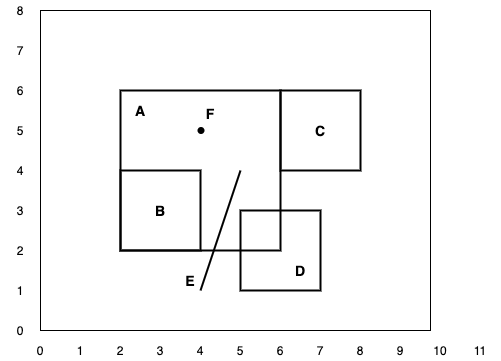
\includegraphics[width=0.5\linewidth]{images/geosparql_example.png}
    \caption{\textit{Illustration of spatial data} van \cite{ogcdocs}}
    \label{fig:illustration_spatial_data}
\end{figure}

\subsection{Terraformer}
Terraformer was een eerste en zeer voor de hand liggende keuze, omdat deze reeds gebruikt werd voor de omzetting van WKT naar GeoJSON. Zo heeft Terraformer een module voor het werken met GeoJSON. De module heet Terraformer Core. Deze module voorziet functies voor onder andere het controleren of een vorm binnen een andere vorm ligt en om te controleren of een vorm een andere vorm snijdt. Dit is welliswaar te beperkt om de volledige ``Simple Features'' familie te implementeren, maar voor de ``sfContains'' en nadien voor zowel de ``sfIntersects'' en de ``sfDisjoint'' functies is dit zeker een goed begin. 

Na het maken van de implementatie, bleken er toch enkele problemen te zijn met de ``contains'' functie van Terraformer. Zo valt onmiddellijk op dat er vele randgevallen zijn die niet correct werken. Enkele voorbeelden daarvan zijn de volgende:
\begin{itemize}
    \item Polygoon ``contains'' lijn: wanneer de lijn van een hoekpunt naar een ander hoekpunt gaat (dus wanneer het een zijde of een diagonaal is), zou dit ``true'' moeten geven, maar dit geeft ``false''.
    \item Polygoon ``contains'' polygoon: wanneer de polygonen een hoekpunt delen (dus deze ligt erin, maar ligt helemaal in de hoek), zou dit ``true'' moeten geven, maar dit geeft ``false''.
\end{itemize}

Om een oplossing te zoeken voor deze randgevallen, moet er teveel code veranderd worden. Aangezien deze randgevallen zeer vaak voorkomen (en aangezien de kans reëel is dat er nog meerdere andere fouten zijn), werd besloten om een andere oplossing te zoeken die meer bruikbaar is voor het geheel, zoals de andere topologische functies.

\subsection{Manueel}
Het eerst volgende idee was om dit manueel op te lossen. Dit leek een logische oplossing, omdat zo alle functies met zekerheid gemaakt kunnen worden en dit met een implementatie die conform is met de OGC standaarden. Hier werd echter vrij snel van afgeweken vanwege de complexiteit. Het uitgevoerde onderzoek wordt hieronder beschreven, opnieuw voor het voorbeeld voor de ``contains'' functie. Hierbij werd ook enkel aandacht gegeven aan de enkelvoudige vormen (dus ``Point'', ``LineString'' en ``Polygon''). De gedachtengang hierbij was dat de meervoudige vorm identiek was, maar zich meerdere keren herhaalt.

\subsubsection{Point}
Bij het beginnen van een eigen implementatie is het het eenvoudigste om te beginnen bij een punt. Hierbij is het namelijk zo dat een punt enkel in een punt ligt wanneer dit punt exact hetzelfde is. Het controleren of een lijn of een polygoon in een punt ligt is nog eenvoudiger, dit is namelijk niet mogelijk (en bijgevolg dus altijd ``false'').  

\subsubsection{LineString}
Het volgende deel is logischerwijs controleren wat binnen een lijn kan liggen. Voor een punt is dit eenvoudig (wiskundig) op te lossen, door voor elk deel van de lijn de richtingscoëfficient uit te rekenen en vervolgens te kijken of het punt op de lijn ligt. Hierbij moet wel opgelet worden, aangezien het deel van de lijn niet oneindig doorloopt. Dit is evenwel eenvoudig op te lossen door te controleren dat de x-coördinaat van het punt tussen de x-coördinaten van de uiteinden van de lijn ligt.

Bij het controleren of een lijn in een andere lijn ligt, kan dezelfde techniek als bij een punt gebruikt worden. Hierbij moet voor elk deel van de mogelijks binnen liggende lijn gecontroleerd worden of de uiteinden op de eerste lijn liggen. Ook moet er gecontroleerd worden of de richtingscoëfficient van beide lijnen in dit deel (het volledige deel) identiek is. Indien deze voorwaarden voldaan zijn, dan ligt de lijn binnen de andere lijn. 

De controle of een polygoon binnen een lijn ligt is overbodig. Dit is namelijk onmogelijk, bijgevolg kan deze functie rechtstreeks ``false'' als uitkomst geven.

\subsubsection{Polygon}
Het laatste en moeilijkste deel is controleren of een vorm binnen een polygoon ligt. Het eerste deel is het controleren of een punt binnen een polygoon ligt. Intuïtief wordt direct gedacht aan het wiskundig beschrijven van een vlak, maar dit is echter niet bruikbaar. Vervolgens kan gecontroleerd worden of het punt onder of boven een lijn ligt, om zo te proberen achterhalen of dit betekent dat het punt binnen de polygoon ligt. Het probleem heeft echter een eenvoudigere oplossing dan dit. Wanneer het punt op een lijn van de polygoon ligt, is meteen geweten dat de ``contains'' functie ``true'' moet weergeven. Wanneer dit niet het geval is, kan een andere techniek gebruikt worden. Zo kan een horizontale lijn getrokken worden, vertrekkend vanuit het punt en helemaal naar rechts (met oneindige lengte). Wanneer nu geteld wordt met hoeveel lijnen van de polygoon deze lijn kruist, is de uitkomst gekend. Het punt ligt namelijk binnen de polygoon wanneer het aantal kruissende lijnen een oneven aantal is. Deze techniek is geïllustreerd in \figureref{fig:polygon_contains_point}.

\begin{figure}
    \centering
    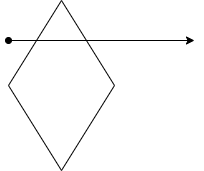
\includegraphics[width=0.5\linewidth]{images/polygon_contains_point.png}
    \caption{Polygon contains point example.}
    \label{fig:polygon_contains_point}
\end{figure}

Het volgende deel is het controleren of een lijn binnen een polygoon ligt. Hiervoor is er opnieuw een techniek. Voor de lijn moet gecontroleerd worden of een punt binnen de polygoon ligt. Indien dit het geval is, moet ook nog eens gecontroleerd worden of de lijn snijdt met een rand van de polygoon. Dit betekent dat elke lijn van de rand van de polygoon gecontroleerd moet worden. Het controleren of lijnen snijden is opnieuw wiskundig aan te pakken, maar hier wordt niet verder op ingegaan. Deze techniek is geïllustreerd in \figureref{fig:polygon_contains_line}.

\begin{figure}
    \centering
    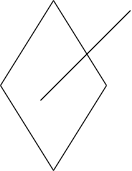
\includegraphics[width=0.3\linewidth]{images/polygon_contains_line.png}
    \caption{Polygon contains line example.}
    \label{fig:polygon_contains_line}
\end{figure}

Het laatste deel hierbij is het controleren of een polygoon binnen een polygoon ligt. Hiervoor zou intuïtief gedacht kunnen worden aan het controleren of alle punten van de (vermoedelijk) binnenste polygoon binnen de andere polygoon liggen. Zoals geïllustreerd in \figureref{fig:polygon_contains_polygon} is dit niet altijd het geval. Dit is enkel mogelijk indien de buitenste vorm convex (= bolvormig) is. Aangezien dit in vele gevallen niet zo is, zou het verlies van performantie zijn om hierop te controleren. Een correcte techniek is echter controleren of één enkel punt van de (vermoedelijk) binnenste polygoon binnen de andere polygoon ligt. Vervolgens volstaat het om te controleren of er een lijn van de rand van de ene polygoon snijdt met een lijn van de rand van de andere polygoon. Indien er snijdende lijnen zijn, zal de ``contains'' functie ``false'' teruggeven. Hierbij wordt ook duidelijk dat deze berekeningen computationeel intensief worden, zeker in het geval van queryen. Dit kan nog verbeterd worden door de lijn intersectie tests te versnellen met het ``\textit{sweep line}'' algoritme, maar hier wordt niet verder op ingegaan. In het voorbeeld in \figureref{fig:polygon_contains_polygon} is de gekleurde polygoon degenen die getest wordt om binnen de andere te liggen.

\begin{figure}
    \centering
    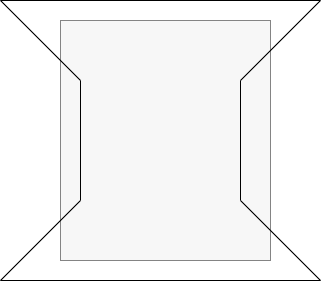
\includegraphics[width=0.3\linewidth]{images/polygon_contains_polygon.png}
    \caption{Polygon contains polygon example.}
    \label{fig:polygon_contains_polygon}
\end{figure}


\subsubsection{Extra moeilijkheden}
De eerder vernoemde technieken zijn al vrij ingewikkeld en dit is slechts voor de ``contains'' functie. Hier zouden nog meerdere andere technieken gebruikt moeten worden om de andere functies te implementeren. Dit wordt nog ingewikkelder wanneer ook rekening gehouden wordt met de veelvoudige vormen zoals ``MultiPoint'', ``MultiLineString'' en ``MultiPolygon''. Hierbovenop is er ook nog geen rekening gehouden met de binnenste ring van de polygonen, die een deel van het vlak excluderen. Dit is nog een extra moeilijkheidsfactor waar rekening mee moet worden gehouden.  

Zo zijn er vele nadelen aan het zelf implementeren hiervan. Een eigen implementatie kan al vele fouten bevatten, bij functionaliteiten zoals dit. Ook moet dit uitvoerig getest worden, wat best door een maximaal aantal gebruikers gebeurt. Bovendien moeten de meest performante algoritmes gebruikt worden, zodat dit bruikbaar is voor queries. Al deze redenen verwerpen het zelf implementeren. Hierna is er overgegaan naar ``Turf.js''.

\subsection{Turf.js}
``Turf.js'' is een modulaire geospatiale engine die gemaakt is in JavaScript. Zo is Turf een JavaScript \textit{library} die werkt aan de hand van GeoJSON. Het is een verzameling van kleine modules, zodat gebruik kan gemaakt worden van exact wat nodig is voor de \textit{use case}. Turf gebruikt naar eigen zeggen de nieuwste algoritmes, wat een pluspunt is voor de performantie. Bovendien heeft Turf een uitgebreide grote comunity die ervoor zorgt dat mogelijke fouten in de implementatie gevonden en opgelost worden. Zo kan een bug opgelost worden door de nieuwste versie binnen te halen.

Turf voorziet vele methoden die gebruikt kunnen worden om zelf verder berekeningen op te doen. Daarnaast heeft Turf al enkele \textit{build in} functies, zoals ``booleanContains'', ``booleanDisjoint'' en ``booleanOverlap''. Deze functies zijn exact wat nodig is. Een overzicht van de functies die gebruikt zijn voor de implementatie van de ``Simple Features'' familie is te zien in \tableref{tab:turf_functions}.

\begin{table}[ht]
    \centering
    \begin{tabular}{ |p{2cm}|p{2cm}|p{8cm}| } 
        \hline
        \rowcolor{TableHeaderColor} GeoSPARQL functie & Turf.js functie & Opmerkingen \\ \hline
        
        \rowcolor{TableColor} sfEquals & booleanEqual & De functie van Turf is volledig conform met de documentatie. \\ \hline

        \rowcolor{TableColor} sfDisjoint & booleanDisjoint & De functie van Turf blijkt volledig conform te zijn met de documentatie van GeoSPARQL. Deze bevat echter een bug waarbij twee evenwijdige en overlappende lijnen toch ``disjoint'' zouden zijn. \\ \hline

        \rowcolor{TableColor} sfIntersects & !booleanDisjoint & Deze functie heeft hetzelfde probleem als sfDisjoint, aangezien deze het inverse is. \\ \hline

        \rowcolor{TableColor} sfTouches & / & Turf heeft nog geen functie die gebruikt kan worden voor deze functionaliteit. \\ \hline

        \rowcolor{TableColor} sfWithin & booleanWithin & De functie van Turf blijkt volledig conform te zijn met de documentatie van GeoSPARQL. Deze bevat echter een bug bij het gebruik van de binnenste ring. \\ \hline

        \rowcolor{TableColor} sfContains & booleanContains & De functie van Turf blijkt volledig conform te zijn met de documentatie van GeoSPARQL. Deze bevat echter een bug bij het gebruik van de binnenste ring. \\ \hline

        \rowcolor{TableColor} sfOverlaps & booleanOverlap & De functie van Turf is niet volledig conform met de documentatie van GeoSPARQL. Het verschil hierbij is dat het voor Turf voldoende is om enkel de borders te laten overlappen, terwijl GeoSPARQL benadrukt dat ook de interiors moeten overlappen. \\ \hline

        \rowcolor{TableColor} sfCrosses & booleanCrosses & De functie ``booleanCrosses'' van Turf zou overeen moeten komen, maar deze heeft andere specificaties waardoor deze niet bruikbaar is.  \\ \hline
    \end{tabular}
    \caption{Implementatie GeoSPARQL functies (Simple Features familie) met ``Turf.js''.}
    \label{tab:turf_functions}
\end{table}